\documentclass[a4paper,oneside,11pt,openany]{book}

\usepackage{../../utils/main-config}
\usepackage{../../utils/discrete-math-macros}


% Document info
\title{
    Дискретная Математика\\
    [1ex]
    \largeСеместр 1 - Осень - 2020
}
\author{
    Конспект составила - Мария Атмажитова\\
    Отредактировал и дополнил - Азим Мурадов
}

% Document
\begin{document}

    \maketitle

    В документе конспект лекций по дискретной математике, прочитанных Татьяной Викторовной Абрамовской 171, 172 и 173 группам МатМех-а СПбГУ в осеннем семестре 2020-2021 учебном года.
    Он, разумеется, неполный, так как это не более чем затеханные записи с лекций.

    Если вам есть чем его дополнить — напишите мне на почту \href{mailto:m.atmazh@yandex.ru}{m.atmazh@yandex.ru}

    В конспекте часто используется сокращение a.k.a. $=$ 'also known as' $=$ \guillemotleft также известный как\guillemotright.
    Оно не является общепринятым для математических текстов, поэтому стоит его упомянуть отдельно.
    Также иногда союз \guillemotleft и\guillemotright ~обозначается значком $\wedge$.

    \tableofcontents


    \chapter[Множества и Разбиения]{Начальная теория множеств и Разбиения (Вводный параграф)}\label{ch:ch-1}


% Множества
\section{Множества}\label{sec:ch-1-sec-1}


\begin{definition}[Наивная теория множеств]
    \begin{compactenum}
        \item Множество однозначно определяется своими объектами и может быть задано простым перечислением. $A = \set{1, \lambda, word, \set{IV, white}}$
        \item Порядок элементов в множестве не имеет значения. $\set{a, b} = \set{b, a}$
        \item Будем говорить, что элемент $a$ принадлежит множеству $A$, или что этот элемент содержится в нём если $A = \set{a, \ldots}$, и будем обозначать это $a \in A$.
        \item Множество может быть задано с помощью предиката. $A = \set{x : P(x)}$ или $A = \set{x \mid P(x)}$ (последнее будет использоваться чаще)
    \end{compactenum}
\end{definition}

\begin{definition}[Подмножество]
    Будем говорить, что множество $A$ является \definiendum{подмножеством} множества $B$,
    или что $B$ является \definiendum{надмножеством} $A$ если каждый элемент в $A$ также содержится в $B$.
    \\[1ex]
    Т.е. $A \subseteq B \coloneqq \forall x \in A \imp x \in B$; $\subseteq$ --- \definiendum{отношение вложения}.
\end{definition}

\begin{sh-proposition}
    $A \subseteq B \land B \subseteq A \iff A = B$
\end{sh-proposition}

\begin{definition}[Собственное подмножество]
    $\subset$ --- \definiendum{отношение строгого вложения} (аналогично \definiendum{собственное подмножество}):
    \\[1ex]
    $A \subset B \coloneqq A \subseteq B \land A \neq B$
\end{definition}

\begin{examples}[Множества и теоретико-множественные записи]
    \begin{compactenum}
        \item $\Phi = \set{1, \lambda, \textrm{слово}, \set{IV, white}}$
        \item $\textrm{Щ} = \set{1, a} \quad \textrm{Ъ} = \set{a, 1}$
        \item $\textrm{слово} \in \Phi \quad \set{\lambda, \textrm{слово}} \subseteq \Phi$
        \item $\set{IV, white} \not\subseteq \Phi$
        \item $\Lambda = \set{\set{IV, white}} \subseteq \Phi$
        \item $\Lambda \subset \Phi$
    \end{compactenum}
\end{examples}

\begin{definition}[Простые опреации над множествами]
    \begin{compactitem}
        \item \definiendum{Объединение множеств}: $A \cup B = \set{x \mid x \in A \lor x \in B}$
        \item \definiendum{Пересечение множеств}: $A \cap B = \set{x \mid x \in A \land x \in B}$
        \item \definiendum{Разность множеств}: $A \setminus B = \set{x \mid x \in A \land x \notin B}$
        \item \definiendum{Симметрическая разность множеств}: $A \symdif B = \p{A \setminus B} \cup \p{B \setminus A}$
    \end{compactitem}
\end{definition}

\begin{sh-designation}[Пустое множество]
    $\varnothing = \set{}$
\end{sh-designation}

\begin{sh-definition}[Множество натуральных чисел]
    $\N = \set{1, 2, 3, \ldots}$
\end{sh-definition}

\begin{sh-designation}[Отрезок натурального ряда]
    $m:n \coloneqq
    \begin{cases}
        \set{m, m + 1, \ldots, n}, & m < n\\
        \set{m}, & m = n\\
        \varnothing, & m > n
    \end{cases}$
\end{sh-designation}

\begin{designation}[Множество множеств]
    $\Lambda = \set{\Lambda_i \mid \forall i \in I}$, где $I$ --- множество индексов, в данном контексте обычно дискретное (то есть конечное или счётное).
\end{designation}

\begin{sh-designation}[Объединение множества множеств]
    $\bigcup \Lambda = \set{x \mid \exists i \in I\ x \in \Lambda_i}$
\end{sh-designation}

\begin{sh-designation}[Пересечение множества множеств]
    $\bigcap \Lambda = \set{x \mid \forall i \in I\ x \in \Lambda_i}$
\end{sh-designation}

\begin{sh-definition}[Булеан]
    \label{Булеан}
    $\2{A}$ --- множество всех подмножеств множества $A$.
    Также называют \definiendum{булеаном}.
\end{sh-definition}

\begin{sh-remark}
    Не надо читать это~\thref{Булеан} как <<два в степени A>>, по крайней мере, на экзамене у Абрамовской так делать точно не стоит.
\end{sh-remark}

\begin{sh-example}
    $\Phi$ задано выше.
    Тогда $\set{1, \lambda} \subseteq \Phi \imp \set{1, \lambda} \in \2{\Phi}$
\end{sh-example}

\begin{sh-remark}
    $\forall A \imp \varnothing \subseteq A, \varnothing \in \2{A}, \varnothing \subseteq \2{A}$
\end{sh-remark}

\begin{sh-definition}[Мощность множества]
    $\abs{A}$ --- число элементов в множестве $A$ или \definiendum{мощность} $A$
\end{sh-definition}

\begin{sh-designation}[Конечное множество]
    $A$ --- конечно $\iffdef \abs{A} < \infty$
\end{sh-designation}

\begin{sh-proposition}[Мощность булеана]
    $\forall A : \abs{A} < \infty \imp \abs{\2{A}} = 2^{\abs{A}}$
\end{sh-proposition}

\begin{proof}
    Для доказательства данного факта воспользуемся методом математической индукции.

    База индукции: $A = \varnothing \imp \abs{A} = 0, \2{A} = \set{\varnothing} \imp \abs{\2{A}} = 1$.

    Переход индукции: пусть $\abs{X} = n + 1$ и известно, что $\forall A : \abs{A} = n \imp \abs{\2{A}} = 2^n$, покажем, что $\abs{\2{X}} = 2^{n + 1}$.
    Поскольку $n \geq 0 \imp \exists x \in X$, рассмотрим $X \setminus \set{x} = \widetilde{X} : \abs{\widetilde{X}} = n \imp \abs{\2{{\widetilde{X}}}} = 2^n$.\\
    $\2{X}=\2{{\widetilde{X}}} \cup \set{\chi\cup\set{x} \mid \chi \in \2{{\widetilde{X}}}}$

    Поскольку $\2{{\widetilde{X}}} \cap \set{\chi\cup\set{x} \mid \chi \in \2{{\widetilde{X}}}} = \varnothing \imp \abs{\2{X}} = \abs{\2{{\widetilde{X}}}} + \abs{\set{\chi\cup\set{x} \mid \chi \in \2{{\widetilde{X}}}}} = 2^n + 2^n = 2^{n + 1}$.
\end{proof}

% Разбиения множеств
\section{Разбиения множеств}\label{sec:ch-1-sec-2}


\begin{definition}[Разбиение мн-в]
    $A \neq \varnothing$, тогда $K$ --- \definiendum{разбиение} $A$, если
    $\begin{cases}
         K \subseteq 2^A,\\
         \bigcup K = A,\\
         \forall k, l \in K \Rightarrow k \cap l = \varnothing,\\
         \varnothing \notin K.
    \end{cases}$
\end{definition}

\begin{definition}[Измельчение разбиения]
    $\sqsupset K, L$ --- разбиения $A$, тогда говорят, что $K$ \definiendum{измельчает} $L$, если $\forall ~k \in K ~\exists ~l \in L: k \subseteq l$.
\end{definition}

\begin{definition}[Произведение разбиений]
    $\sqsupset K, L$ --- разбиения $A$, тогда \definiendum{произведение разбиений} --- наибольшее по включению разбиение $A$, измельчающее $K$ и $L$.
\end{definition}

\begin{sh-proposition}
    Произведение разбиений существует.
\end{sh-proposition}

\begin{proof}
    Неформально: смотрим картинку и радуемся жизни

    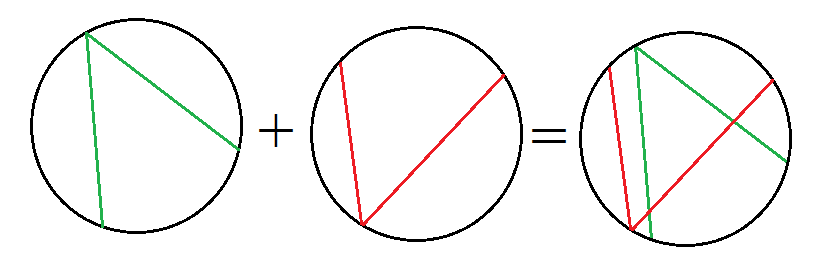
\includegraphics[scale=0.5]{res/произведение разбиений}

    Чуть более формально: пересекаем все $X \in K$ со всеми $Y \in L$ и выкидываем пустые множества, получаем то, что надо.

    Ещё более формально: пусть $B = \{X\cap Y : X\in K, Y\in L, X\cap Y \neq \varnothing\}$.

    $B$ — разбиение $A$, так как $\forall ~b \in B ~b \in 2^A, b \neq \varnothing, \forall ~a \in A ~\exists! ~b\in B: a\in b$.

    Пусть $C$ --- тоже разбиение $A$, измельчающее $K$ и $L$, покажем, что $C$ измельчает и $B$.

    Пусть $c \in C \Rightarrow ~\exists ~X \in K ~\exists ~Y \in L: c\subseteq K$ и $c \subseteq L \Rightarrow c \subseteq K \cap L \Rightarrow ~\exists ~b=K\cap L \in B: c\subseteq b$.

    При желании можно накрутить ещё формализма, но так ли оно надо?
\end{proof} % Начальная теория множеств и Разбиения (Вводный параграф)
    % \chapter{Бинарные отношения}\label{ch:ch-2}


% Кортежи
\section{Кортежи}\label{sec:ch-2-sec-1}

% Бинарные отношения
\section{Бинарные отношения}\label{sec:ch-2-sec-2}

\begin{definition}[Свойства бинарных отношений]
    Пусть $A$ --- множество, $R \subseteq A \times A$, тогда:

    \begin{compactitem}
        \item $R$ \definiendum{рефлексивно}, если $\forall ~a \in A (a, a) \in R$.
        \item $R$ \definiendum{симметрично}, если $\forall ~a, b \in A (a, b) \in R \Leftrightarrow (b, a) \in R$.
        \item $R$ \definiendum{транзитивно}, если $\forall ~a, b, c \in A (a, b) \in R \wedge (b, c) \in R \Rightarrow (a, c) \in R$.
        \item $R$ \definiendum{антирефлексивно}, если $\forall ~a \in A (a, a) \notin R$.
        \item $R$ \definiendum{антисимметрично}, если $\forall ~a \in A (a, b) \in R \wedge (b, a) \in R \Rightarrow a = b$.
        \item $R$ \definiendum{антитранзитивно}, если $\forall ~a, b, c \in A (a, b) \in R \wedge (b, c) \in R \Rightarrow (a, c) \notin R$.
        \item $R$ \definiendum{асимметрично}, если $\forall ~a \in A (a, b) \in R \Rightarrow (b, a) \notin R$.
    \end{compactitem}
\end{definition}

% Отображения
\section{Отображения}\label{sec:ch-2-sec-3}

% Отношения порядка
\section{Отношения порядка}\label{sec:ch-2-sec-4}


\begin{definition}[Отношение частичного порядка]
    $R$ --- \definiendum{отношение частичного порядка} на $A$, если $R$ рефлексивно, транзитивно и антисимметрично.
\end{definition}

\begin{sh-designation}
    Будем сокращать "частично упорядоченное множество"\ до \definiendum{чум} или \definiendum{poset} (partially ordered set).
\end{sh-designation}

\begin{sh-example}
    Отношение вложенности в множество ($\subseteq$).
\end{sh-example}

\begin{theorem}
    Пусть $A$ --- множество, а $R$ --- частичный порядок на $A$, тогда $\exists ~\Lambda \subseteq A \times 2^A$ --- отображение, т.ч. $(a, b) \in R \Leftrightarrow \lambda(a) \subseteq \lambda(b) \forall ~a, b \in A$.
\end{theorem}

\begin{proof}
    $\forall ~a \in A \lambda(a) = \{x \in A : (x, a) \in R\}$

    \quad $S = \{\lambda(a) | a \in A\}$

    \quad $\Lambda = \{(a, \lambda(a)) | a \in A\}$ --- отношение на $A \times S$ (сюръективно по построению, доказательство инъективности приведено ниже)

    Докажем, что $\lambda(a) = \lambda(b) \Leftrightarrow a = b$.

    \fbox{$\Leftarrow$} очевидно

    \fbox{$\Rightarrow$} пусть $\lambda(a) = \lambda(b)$; $(a, a) \in R$, так как $R$ рефлексивно $\Rightarrow a \in \lambda(b) \Rightarrow (a, b) \in R$; аналогично $(b, a) \in R \Rightarrow b = a$.

    Пусть $(a, b) \in R \Leftrightarrow \forall ~x \in A: (x, a) \in R (x, b) \in R \Leftrightarrow \forall ~x \in \lambda(a) x \in \lambda(b) \Leftrightarrow \lambda(a) \subseteq \lambda(b)$.
\end{proof}


\begin{sh-example}
    $A = \{1, 3, 4, 6, 8, 12\}$, $D = \{(a, b): b | a, a, b \in A\}$ --- частичный порядок, $\lambda(a)$ --- делители $a$.
\end{sh-example}

\begin{definition}[Отношение строгого частичного порядка]
    $R$ --- \definiendum{отношение строгого частичного порядка}, если $R$ асимметрично и транзитивно.
\end{definition}

\begin{definition}
    [Отношение (строгого) линейного порядка]
    $A$ (строго) частично упорядочено $R$, $\forall ~a, b \in A (a, b) \in R \vee (b, a) \in R \vee a = b \Rightarrow R$ --- \definiendum{отношение (строгого) линейного порядка} на $A$.
\end{definition}

\begin{examples}
    \begin{compactenum}
        \item $\subseteq$ --- частичный, но не линейный порядок
        \item $\leq$ --- линейный порядок
        \item $<$ --- строгий линейный порядок.
    \end{compactenum}
\end{examples}

\begin{definition}
    Пусть $A$ частично упорядочено относительно $R$, тогда:

    \begin{compactitem}
        \item $m \in A$ --- \definiendum{минимальный} элемент, если $\forall ~x \in A (x, m) \notin R$.
        \item $m \in A$ --- \definiendum{наименьший} элемент, если $\forall ~x \in A\backslash\{m\} (m, x) \in R$.
        \item $M \in A$ --- \definiendum{максимальный} элемент, если $\forall ~x \in A (M, x) \notin R$.
        \item $M \in A$ --- \definiendum{наибольший} элемент, если $\forall ~x \in A\backslash\{M\} (x, M) \in R$.
    \end{compactitem}
\end{definition}

% Топологическая сортировка
\section{Топологическая сортировка}\label{sec:ch-2-sec-5}

В этом параграфе под фразой \guillemotleftчастичный порядок\guillemotright ~будет подразумеваться \guillemotleftчастичный порядок или строгий частичный порядок\guillemotright.

\begin{lemma}[О сужении бинарного отношения]
    Пусть $R$ — рефлексивное / антирефлексивное / симметричное / антисимметричное / асимметричное / транзитивное / антитранзитивное отношение на $A$, тогда $\forall ~X \subseteq A ~R(X)=R\cap X^2$ (a.k.a. \textbf{сужение} $R$ на $X$) — тоже.
\end{lemma}

\begin{sh-proof}
    Тривиально и предоставляется читателю в качестве лёгкого упражнения.
\end{sh-proof}

\begin{lemma}[О существовании минимального элемента]
    Во всяком конечном частично упорядоченном непустом множестве существует минимальный элемент.
\end{lemma}

\begin{proof}
    Кратко: индукция по мощности множества.

    Подробно: для доказательства данной леммы воспользуемся методом математической индукции.

    \textit{База индукции:} $X = \{x\}$. Минимальный элемент очевидно существует и равен $x$.

    \textit{Переход индукции:} пусть $|X| = n + 1, n \geq 1$ и известно, что в любом множестве мощностью $n$ существует минимальный элемент. Тогда выберем $x \in X$ и рассмотрим $X' = X \backslash \{x\}$. По предположению индукции в $X'$ есть минимальный элемент, обозначим его $x_0$. Если $(x, x_0) \in R$, то $x$ — минимальный элемент $X$, так как $\forall ~x' \in X (x', x) \notin R$ (в противном случае $(x', x_0) \in R$, из чего следует, что $x_0$ — не минимальный элемент $X'$). Иначе $x_0$ остаётся минимальным элементом.
\end{proof}

\begin{sh-definition} [Топологическая сортировка]
    poset $A$ отн. $R$ — такой лин. порядок $Q$, что $R \subseteq Q$.
\end{sh-definition}

\begin{theorem}
    У любого конечного частично упорядоченного относительно $R$ множества $A$ существует топологическая сортировка.
\end{theorem}

\begin{proof}
    Конструктивное док-во (чтобы доказать существование чего-нибудь, предъявим нечто и покажем, что это именно то, что мы ищем). Рассмотрим частный случай: $A = \varnothing$. Очевидно, что тогда топологическая сортировка существует и равна $\varnothing$. Теперь предположим, что $A \neq \varnothing$. Для начала упорядочим элементы $A$. Для этого воспользуемся методом математической индукции, но не совсем. Поскольку $A$ непустое, в нём (по лемме 2) существует минимальный элемент. Обозначим его за $m_0$, а само множество $A$ за $A_0$.

    Пусть $A_i \backslash \{m_i\} \neq \varnothing$. Тогда $A_{i + 1} = A_i \backslash \{m_i\}$, $m_{i+1} = min A_i$. Заметим, что $A_{i+1} \subset A_i \Rightarrow A_j \subset A_i$ при $i < j$.

    Обозначим $Q = \{(m_i, m_j) : i \leq j\}$, если $R$ — частичный порядок, и $Q = \{(m_i, m_j) : i < j\}$, если $R$ — строгий частичный порядок. Покажем, что $Q$ — искомая топологическая сортировка.

    Очевидно, что рефлексивность / антирефлексивность следует из построения $Q$. Антисимметричность тоже. Транзитивность тривиальна. Линейность тоже. Следовательно, $Q$ — отношение линейного порядка на $A$. Покажем, что $R \subseteq Q$.

    Предположим противное: существуют $i > j$ такие, что $(m_i, m_j) \in R$. Тогда $m_i \notin A_j$, что противоречит тому, что $A_i \subset A_j$, что следует из построения $A_i$ и $m_i$. Соответственно, $R \subseteq Q$ и всё хорошо.
\end{proof}

\begin{sh-remark}
    $R^{-1} = \{(y, x) : (x, y) \in R\}$ — частичный порядок, если $R$ — частичный порядок $\Rightarrow min R = max R^{-1}$.
\end{sh-remark}

\begin{sh-remark}
    $A$ — строго poset относительно $R \Rightarrow Q$ — строгий линейный порядок.
\end{sh-remark} % Бинарные отношения
    % \include{content/ch-3}
    % \include{content/ch-4}
    % \include{content/ch-5}
    % \include{content/ch-6}
    % \include{content/ch-7}

\end{document}